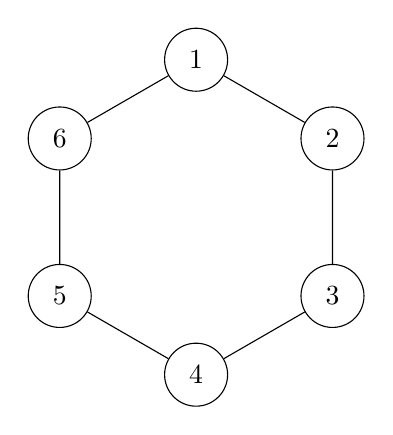
\begin{tikzpicture}[
    vertex/.style={
        circle,
        draw,
        minimum size=8mm,
        inner sep=0pt
    }
]

\foreach \i in {1,...,6} {
    \node[vertex] (\i) at ({90-60*(\i-1)}:2cm) {\i};
}

\draw (1) -- (2) -- (3) -- (4) -- (5) -- (6) -- (1);

\end{tikzpicture}
\quad
\begin{tikzpicture}[
    vertex/.style={
        circle,
        draw,
        minimum size=8mm,
        inner sep=0pt
    },
    arrow/.style={
        -{Stealth},
        thick,
        bend right=20
    }
]

\foreach \i in {1,...,6} {
    \node[vertex] (\i) at ({90-60*(\i-1)}:2cm) {\i};
}

\draw[arrow] (1) to (6);
\draw[arrow] (6) to (5);
\draw[arrow] (5) to (4);
\draw[arrow] (4) to (3);
\draw[arrow] (3) to (2);
\draw[arrow] (2) to (1);

\end{tikzpicture}